\subsection{Aufbau}
In Abbildung \ref{fig:Aufbau} ist der Aufbau eines Geiger-Müller-Zählrohrs zu sehen. Es besteht aus einer Anode und einer Kathode, die zusammen einen Zylinderkondensator bilden. Das Elektrische Feld ist radialsymmetrisch
\begin{align}
	E(r) = \frac{U}{r\ln(\frac{r_\text{k}}{r_\text{a}})} \ .
\end{align}
\begin{figure}[h!]
	\centering
	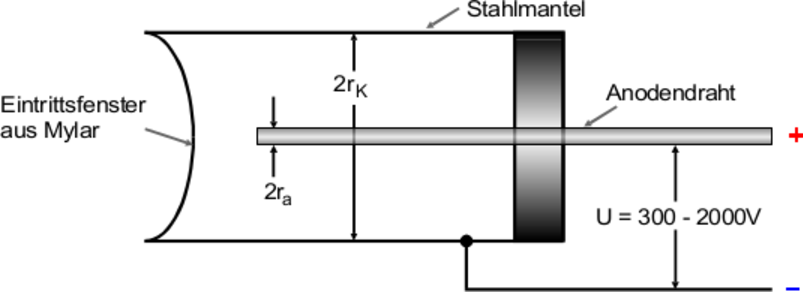
\includegraphics[width=0.7\textwidth]{Aufbau.pdf}
	\caption{Grundsätzlicher Aufbau eines Geiger-Müller-Zählrohrs \cite{\V}}
	\label{fig:Aufbau}
\end{figure}
Außerdem ist der Kondensator mit einem Gas gefüllt.
\subsection{Funktionsweise}
\todo[color=red,inline]{Das Teilchen ist doch geladen, wird also durch das elektrische Feld zum Draht oder zum Zylinder gezogen. Was ist, wenn das Teilchen an einem der beiden ankommt und noch Energie übrig hat? Bzw. es wird durch das Feld ja sogar beschleunigt. Stößt es sich an der Anode/Kathode ab und bewegt sich weiter? Geht die Energie verloren? Kann das Teilchen dann, wenn es sich nicht mehr fortbewegt auch noch ionisieren? \\ Je nach dem wäre die Energie nicht mehr proportional zur Anzahl.}
Ein geladenes Teilchen, das in das Zählrohr eindringt, ionisiert die Gasatome. Dabei verliert es jedes Mal einen (sehr kleinen) Teil seiner Energie und bewegt sich solange weiter fort, bis seine gesamte Energie aufgebraucht ist. Bei jeder Ionisation entstehen ein Elektron und ein positiv geladener Atomrumpf. Die Anzahl dieser Ionenpaare ist proportional zur ursprünglichen Teilchenenergie.
\subsubsection*{Spannungsabhängigkeit}
Was nach der Ionisation geschieht, hängt von der angelegten Spannung ab. Es können die nachfolgenden Bereiche, die in Abbildung \ref{fig:DependenceVoltage} dargestellt sind, unterschieden werden.
\begin{itemize}
	\item[I] Ist die Spannung klein, reicht die Beschleunigung des elektrischen Felds nicht aus, um die Elektronen bis zur Anode zu bringen. Die meisten rekombinieren vorher mit den Atomrümpfen. Mit ansteigender Spannung sinkt die Rekombinationswahrscheinlichkeit schnell ab, sodass bald alle erzeugten Elektronen am Draht ankommen.
\end{itemize}